\chapter{Methods}\label{chap:methods}
    \paragraph{}This research dives into the complexities of embedding byte sequences, focusing particularly on the extraction of structures containing SSH keys for machine learning purposes. The varied uses of OpenSSH introduce distinct challenges due to potential variations in the created embeddings. Given the wide array of SSH key dimensions and OpenSSH's intricate operations, maintaining the embeddings' stability and consistency is vital. In this methodological section, we will detail various embedding methods, present a framework for their assessment through a classifier model, and suggest another strategy to verify the embeddings' coherence between the different OpenSSH usage and key sizes.

    \section{hardware}
        \paragraph{}My primary workstation is an \textit{Aspire 5} laptop, equipped with:
        \begin{itemize}
            \item \textbf{CPU:} 11th Gen Intel i5-1135G7 (8) @ 4.200GHz 
            \item \textbf{GPU:} Intel TigerLake-LP GT2 [Iris Xe Graphics]
            \item \textbf{Memory:} 16GB
        \end{itemize}
        \paragraph{}However, this laptop, despite its decent specifications, proved inadequate for processing the entire dataset. Simple machine learning experiments using a Python script would have stretched over a week. Even when we transitioned to more optimized Rust programs, the processing time exceeded 10 hours. While I managed to run minor tasks and scripts on this laptop, the bulk of the experiments necessitated a more powerful server.
        
        \paragraph{}Recognizing this need, I was granted access to a high-performance development server in the later stages of the thesis, around August 2023. The server, an \textit{AS-4124GS-TNR}, boasts the following specifications:
        \begin{itemize}
            \item \textbf{CPU:} 2x AMD EPYC 7662 (256) @ 2.000GHz
            \item \textbf{GPU:} NVIDIA Geforce RTX 3090 Ti
            \item \textbf{RAM:} 512GB DDR4 3200MHz
        \end{itemize}
        \paragraph{}Operating on \textit{Ubuntu 20.04.6 LTS}, this server became the primary platform for the machine learning experiments, given its superior computational capabilities compared to the \textit{Aspire 5} laptop. This invaluable resource was generously provided by the Department of Computer Science at \textit{Universität Passau}, particularly under the guidance of the Chair of Data Science led by Prof. Dr. Michael Granitzer. I extend my sincere appreciation for their unwavering support.
        

    \section{Dataset}
        \paragraph{}The dataset at the core of this thesis, as previously introduced (see \ref{seq:background:dataset}), consists of heap dump raw files related to different OpenSSH use cases and versions. Each heap dump file is paired with a JSON annotation file created by the dataset's creators. These JSON files provide extra information about the heap dump, especially regarding encryption keys. In this section, we will explain our exploration of the dataset, aiming to better comprehend its content and nuances.

        \subsection{Origin}
            \paragraph{}The dataset is derived from heap dumps that capture various OpenSSH usage scenarios. These scenarios encompass four distinct SSH interactions: a straightforward client connection to the server followed by an immediate exit, port-forwarding, secure copying, and SSH shared connection. The heap dumps span different OpenSSH versions and a range of key sizes, from 16 to 64 bytes. These dumps were generated using the SmartKex tool \cite{fellicious_smartkex_2022}. The data collection was conducted on a mini PC equipped with an AMD Ryzen 5500U processor, 16GB of RAM, and a 1TB NVMe SSD, running Debian 11 as its operating system.

        \subsection{Estimating the dataset balancing for key prediction}
            \paragraph{}In this part, our primary objective was to assess the balance of the dataset for key prediction and identify the challenges associated with it.

            \paragraph{}To begin, we aimed to gain an understanding of the dataset's scale. We utilized a code snippet \ref{methods:code:count_all_dataset_files} to count all the files within the dataset, revealing a total of 208,745 files. However, it was imperative to recognize that JSON files, which served as annotation files, were not to be considered part of the raw bytes for embedding. Consequently, these JSON files were excluded from our count to provide a more accurate representation of the dataset's size.

            \begin{lstlisting}[caption={Count all dataset files}, label=methods:code:count_all_dataset_files, language=bash]
            find . -type f | wc -l
            \end{lstlisting}

            \paragraph{}Following this, we employed another code snippet \ref{methods:code:count_raw_files} to specifically count the heap dump raw files, excluding JSON files. This count indicated a total of 103,595 heap dump raw files, which constituted the primary focus of our analysis.

            \begin{lstlisting}[caption={Count heap dump raw dataset files}, label=methods:code:count_raw_files, language=bash]
            find . -type f -name "*.raw" | wc -l
            \end{lstlisting}

            \paragraph*{}To gain further insights into the dataset, we determined its size while excluding annotation files \ref{methods:code:get_dataset_size}. The calculated dataset size amounted to 18,067,001,344 bytes.

            \begin{lstlisting}[caption={Get the size of the dataset}, label=methods:code:get_dataset_size, language=bash]
            find . -type f -name "*.raw" -exec du -b {} + | awk '{s+=$1} END {print s}'
            \end{lstlisting}

            \paragraph{}Considering the nature of the dataset, which featured a maximum of six keys per file, each with a maximum size of 64 bytes, we conducted a rough estimate. We determined that the maximum number of bytes relevant for searching across the dataset was $6 * 64 * 103595 = 39 780 480$ . This calculation accounted for approximately 0.22\% of the dataset's total size.

            \paragraph{}Lastly, it is crucial to acknowledge that the dataset exhibited a significant imbalance and is very large. To address this challenge effectively, strategies were implemented to ensure robust, unbiased analyses, and scalability.
        \subsection*{Annotations}
            \paragraph{}The annotations files are essential to understand the data and how best to utilize them for the study. Each heap dump corresponds to one specific JSON file. To view the contents of these JSON files in a more organized manner, one can reference the method provided at \ref{methods:code:pretty_print_json}. For a clearer understanding, an extract of the JSON annotation from the file located at \path{./Training/client/V_7_8_P1/16/13116-1644920217.json} is available at \ref{methods:code:annotation_extract}.

            \begin{lstlisting}[caption={pretty print JSON}, label=methods:code:pretty_print_json, language=bash]
                python3 -m json.tool file.json
            \end{lstlisting}
            \begin{lstlisting}[language=json, caption={An extract of the JSON annotations}, label=methods:code:annotation_extract]
            {
                /* file ./Training/client/V_7_8_P1/16/13116-1644920217.json*/
                "SSH_STRUCT_ADDR": "5619dd7e5570",
                "SESSION_STATE_ADDR": "5619dd7e5df0",
                "KEY_A_ADDR": "5619dd807f40",
                "KEY_A_LEN": "12",
                "KEY_A_REAL_LEN": "12",
                "KEY_A": "34fbe182e76c49a617a93e2e",
                /*...*/
                "KEY_E_ADDR": "5619dd808000",
                "KEY_E_LEN": "0",
                "KEY_E_REAL_LEN": "0",
                "KEY_E": "",
                "KEY_F_ADDR": "5619dd807fd0",
                "KEY_F_LEN": "0",
                "KEY_F_REAL_LEN": "0",
                "KEY_F": "",
                "HEAP_START": "5619dd7e3000"
            }
            \end{lstlisting}

            \paragraph{}Within these annotation files, several critical pieces of information are present. The ``SSH\_STRUCT\_ADDR'' and ``SESSION\_STATE\_ADDR'' denote the addresses of vital openSSH \glspl{structure}. These addresses are pivotal in gauging the embedding coherence across different openSSH uses and key sizes. If the embeddings of these \glspl{structure} display similarity across various key sizes and openSSH usages, it signifies the embedding's coherence.

            \paragraph{}Other significant annotations such as ``KEY\_A\_ADDR'', ``KEY\_A\_LEN'', ``KEY\_A\_REAL\_LEN'', and ``KEY\_A'' detail the address, length, and value of the key A. In general, six of these annotations can be found for each heap dump. Notably, the ``HEAP\_START'' annotation, along with the length of the heap dump, is of paramount importance. This annotation signifies the starting address of the heap dump. This information not only aids in pinpointing addresses in the heap dump for \glspl{structure} and \glspl{pointer}, but also refines the heuristic used in detecting \glspl{pointer} \ref{seq:background:pointers_and_structures}. By leveraging the ``HEAP\_START'' information, one can verify if a \gls{pointer} is pointing within the heap dump boundaries. As a practical illustration, deducing the address of key A within the heap dump can be achieved by subtracting ``HEAP\_START'' from ``KEY\_A\_ADDR''.

            \paragraph{}However, it's noteworthy that some of these annotation files may be corrupted. Therefore, it's imperative to verify the integrity of each file before its use. In instances where keys are corrupted, such as "KEY\_E" and "KEY\_F" having no recorded values in the extract found at \ref{methods:code:annotation_extract}, it's advised either to remove the corrupted keys or discard the entire file if the data cannot be salvaged. Armed with this understanding, the next logical step would be to leverage this dataset to formulate embeddings and subsequently evaluate their performance.

        \subsection{Malloc header usage and structures detection}
            \paragraph{}As discussed in \ref{seq:background:pointers_and_structures}, subsequent to an initial 8-byte block of zeros, we anticipate the allocation of the first data structure at the heap's commencement. As illustrated in \ref{fig:methods:malloc_header_detection_heap_start}, this data structure spans a size of $ 5102000000000000_{16LE} $ (in little-endian hexadecimal notation) or $ 593_{10} $ bytes. The presence of an odd number arises from the \acrshort{lsb} being set to 1, signifying that the block is allocated (as a flag). Consequently, the actual size of the structure is $ 593_{10} - 1_{10} = 592_{10} $ bytes, which aligns with an 8-byte boundary.

            \begin{figure}[H]
                \centering
                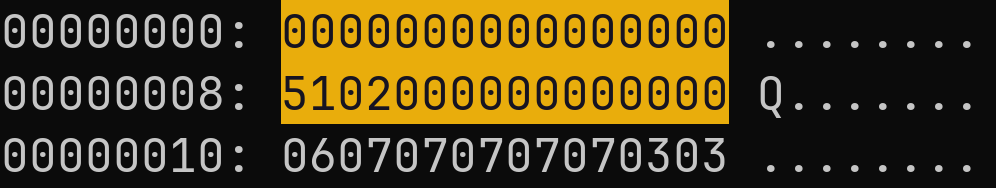
\includegraphics[width=16cm]{background/structure_examples_1010-1644391327-heap_potential_malloc_header_highlight_heap_start.png}
                \caption{Attempt at malloc header detection in \textit{Training/basic/V\_7\_8\_P1/16/5070-1643978841-heap.raw}, at heap start.}
                \label{fig:methods:malloc_header_detection_heap_start}
            \end{figure}

            \paragraph{}Given the allocator's sequential chunk allocation approach, the subsequent chunk's anticipated allocation address is calculated as $ 5102000000000000_{16LE} + 592_{10} + 8_{10} $. The additional 8 accounts for the malloc header block, resulting in an address of $ 5882193a34560000_{16LE} $.
        
            \paragraph{}In vim, since the address start at 0, we have to look at $ 592_{10} + 8_{10} = 258_{16} $. Let's have a look there \ref{fig:methods:malloc_header_detection_0x250}:
    
            \begin{figure}[H]
                \centering
                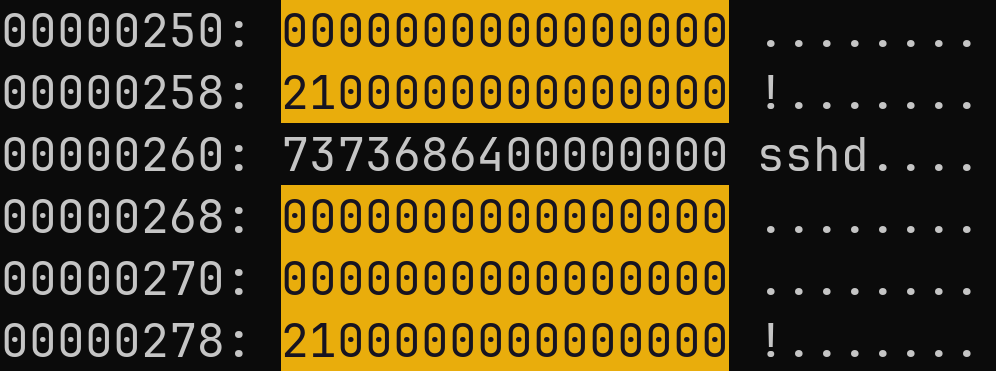
\includegraphics[width=16cm]{background/structure_examples_1010-1644391327-heap_potential_malloc_header_highlight_0x250.png}
                \caption{Attempt at malloc header detection in \textit{Training/basic/V\_7\_8\_P1/16/5070-1643978841-heap.raw}, at index $ 592_{10} = 250_{16} $.}
                \label{fig:methods:malloc_header_detection_0x250}
            \end{figure}
    
            \paragraph{}At this point, we observe a zero block, succeeded by a potential malloc header at address $ 258_{16} $. By replicating this process, we can devise an algorithm to identify malloc headers, and consequently, the structures within the heap dump file.
    
            \begin{algorithm}[H]
                \caption{Malloc Header Detection Algorithm}
                \begin{algorithmic}[1]
                \Procedure{MallocHeaderDetection}{$\text{heapDumpFile}$}
                    \State $\text{position} \gets 0$
                    \While{$\text{position} < \text{FileSize}(\text{heapDumpFile})$}
                        \State $\text{block} \gets \text{Read8Bytes}(\text{heapDumpFile, position})$
                        \If{$\text{block} \neq 0$}
                            \State $\text{size} \gets \text{ConvertToSize}(\text{block}) - 1$ \Comment{$-1$ due to the flag}
                            \State \textbf{Assert} $ \text{size} \mod 8 = 0$ \Comment{Check if the size is 8-bytes aligned}
                            \State $\text{position} \gets \text{position} + 8 + \text{size}$ \Comment{Leap over data structure. + 8 for the header.}
                        \Else
                            \State $\text{position} \gets \text{position} + 8$
                        \EndIf
                    \EndWhile
                \EndProcedure
                \end{algorithmic}
            \end{algorithm}
    
            \paragraph{}The underlying concept of the malloc header detection algorithm is straightforward. Beginning at the start of the heap dump file, we search for the initial non-zero block. Subsequently, we infer that the following block represents a malloc header. This block is converted into a size, allowing us to skip over both the data structure and its header. This procedure continues iteratively until the file's conclusion.
    \section{Embeddings}
        \paragraph{}From the Zenodo dataset\ref{seq:background:dataset}, we've isolated distinct memory structures within the raw heap dump files. These structures possess diverse sizes, necessitating the use of an embedding method for classification. Fortunately, a distinguishing feature of each memory structure is the presence of a header, containing vital information such as the structure's size in bytes. To precisely pinpoint the boundaries of each memory structure, we sequentially parse through the raw heap dump files. Beginning the parsing process from the first non-null byte, identified as the header, serves as a marker for the initiation of a new structure. The size data within this header is then leveraged to calculate the exact length of the structure, allowing for the extraction of its entire raw byte data while determining the start of the subsequent one.
        
        \paragraph{}Our next objective centers on the conversion of raw byte data into fixed-size embeddings (\ref{seq:background:traditional_statistical_embedding}, \ref{seq:background:deep_learning_models_for_raw_byte_embedding}), a pivotal step in preparing them for utilization in machine learning applications. Ensuring uniformity in embedding size across all memory structures holds paramount significance. Consistency in embedding dimensions is vital to empower machine learning algorithms for efficient data processing and analysis. This uniformity not only simplifies the integration of memory structures with varying sizes into a coherent classification framework but also acts as a defense against the adverse effects of the curse of dimensionality—a phenomenon that can introduce computational complexities and heighten the risk of overfitting in high-dimensional data spaces. Striking this equilibrium is essential, achieved by maintaining reasonably low embedding dimensions, fostering both efficient data processing and the preservation of essential information within the raw byte data. It's important to note that initially, each embedding will include the structure's file and the structure's address in the file. However, these details will be removed during the machine learning phase (quality or coherence) as the embedding aims to be free of key size or OpenSSH uses. Their presence will serve as a means to test coherence later in our analysis.

    \section{Embedding quality}
        \paragraph{} Transitioning our focus, we now delve into evaluating the quality of the embeddings. To ensure fairness and comparability among the embeddings, we employ the Pearson correlation method \ref{seq:background:correlation_tests} to limit the selection to the top 8 correlations, thereby narrowing down our analysis to the most influential features. The dataset is notably imbalanced \ref{seq:background:imbalanced_data}, primarily stemming from the rarity of memory structures containing SSH keys, our specific target of interest, within the overall dataset. This rarity results in a significant class imbalance, where the majority of memory structures do not contain SSH keys. To counteract potential bias toward the majority class, we will implement the \acrfull{smote} as a resampling strategy, enabling our model to accurately classify both majority and minority classes. We will then employ a Random Forest model \ref{seq:background:machine_learning}, renowned for its robustness and suitability for high-dimensional data, to carry out the classification task. Our evaluation will rely on metrics such as precision, recall, F1 score, and others to identify the most effective representation for precise classification.

    \section{Embedding coherence}
        \paragraph{}After completing the classification task, our focus shifts to evaluating the coherence of the embedding across different applications of OpenSSH and various key sizes. To accomplish this, we will utilize a clustering model, specifically DBSCAN, which is well-suited for scenarios where the number of clusters is uncertain. Our objective is to determine if the formed clusters demonstrate coherence, signifying the proximity of memory structures containing SSH keys. This analysis also encompasses an assessment of the underlying embedding method's consistency across various uses of SSH and key sizes, illustrating its ability to capture significant patterns and relationships related the the SSH keys.

        \paragraph{}In the following section, we will delve deep into the methodologies and techniques utilized to construct these embeddings, offering a comprehensive insight into the fundamental building blocks of our study.